\documentclass{beamer}
% AnnArbor  Antibes  Bergen  Berkeley  Berlin  Boadilla  CambridgeUS  Copenhagen  Darmstadt  Dresden  Frankfurt  Goettingen  Hannover  Ilmenau  JuanLesPins  Luebeck  Madrid  Malmoe  Marburg  Montpellier  PaloAlto  Pittsburgh  Rochester  Singapore  Szeged  Warsaw  boxes  default 
\mode<presentation>
{
  \usetheme{Antibes}
  \setbeamercovered{transparent}
}

\usepackage[english]{babel}
\usepackage{times}
\usepackage{graphicx}           
\usepackage{xeCJK}       
\usepackage{fontspec}
\setsansfont{SimSun}

\title[南京大学本科毕业设计] 
{状态图自动化建模和模型验证项目(M\&MC)}

\subtitle
{状态图图形化模块的设计与实现}

\author[Author] 
{吴继鹏}

\institute[Universities of Somewhere and Elsewhere] 
{
  南京大学软件学院\\
  规格技术研究小组
}

\date[AFP 2003]
{Final Presentation, 2015}

\subject{Theoretical Computer Science}
\AtBeginSubsection[]
{
  \begin{frame}<beamer>{Outline}
    \tableofcontents[currentsection,currentsubsection]
  \end{frame}
}
\begin{document}

\begin{frame}
  \titlepage
\end{frame}

\begin{frame}{Outline}
  \tableofcontents
\end{frame}

\section{Abstract}
\begin{frame}{这篇报告包括:}
  \begin{itemize}
  \item 支持M\&MC项目的形式化规格方法以及相关理论背景 \pause
  \item M\&MC的项目背景、需求分析和概要设计 \pause
  \item 对基于状态机模型的形式化类规格进行可视化建模的详细设计与实现 \pause
  \end{itemize}
\end{frame}  

\section{基于状态机模型数据抽象的形式化规格方法}
\subsection{相关研究与理论基础}
\begin{frame}{形式化规格的类别}
  \begin{itemize}
  \item 固定原则(fixed discipline), $s := s∪i$  \pause
  \item 任意原则(arbitrary discipline), $insert(s,i)$  \pause
  \item 状态机模型 \pause
  \item 公理化表示 \pause
  \item 代数定义, 少量公理+功能定义 \pause
  \end{itemize}
\end{frame}  
\begin{frame}{形式化规格的质量属性}
  \begin{itemize}
  \item 形式化 \pause
  \item 可构建性 \pause
  \item 最小化 \pause
  \item 应用广度 \pause
  \item 可拓展性 \pause
  \end{itemize}
\end{frame}  
\begin{frame}{其他相关研究}
  \begin{itemize}
  \item inspector,mutator(需要注释的方法) \pause
  \item DBC(依赖于实现) \pause
  \item Statecharts(Harel) \pause
  \end{itemize}
\end{frame}  

\subsection{我们的形式化规格方法}
\begin{frame}{M\&MC中类的状态图模型定义}
  \begin{itemize}
  \item $C=(S, S_0, T)$ \pause
  \item $S={s_1, s_2, \ldots, s_n}(n≥0)$ \pause
  \item $s_i={R_i(v_1), R_i (v_2), \ldots, R_i (v_k)}$ 这已经是抽象化的状态了,一个状态可以包含若干种绝对状态,即由状态变量取值决定的状态。 \pause
  \item $T={t_1, t_2, \ldots, t_m}(m≥0)$, 其中 $t_i$是一个S到S的映射函数。一个transition$t_i$被规格化为(spre, spost, M, C)。\pause
  \end{itemize}
\end{frame}
\begin{frame}{实现者具体定义状态}
  \begin{itemize}
  \item 状态的具体定义依赖于实现,由实现者实现一个purity方法返回状态。
  \end{itemize}
  \begin{figure}[H]
  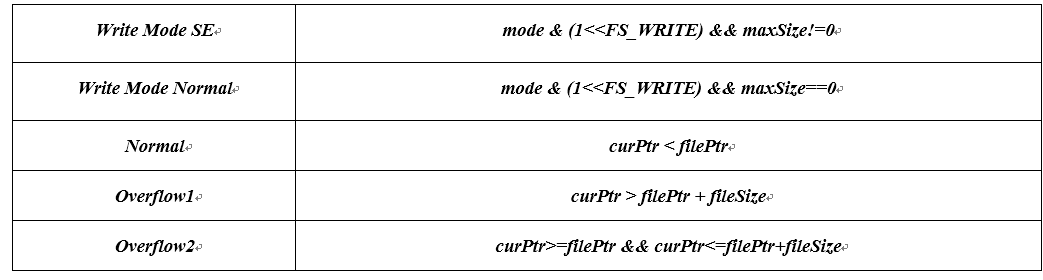
\includegraphics[width=3.6in]{img/1.PNG}
  \end{figure}
\end{frame}
\begin{frame}{状态图模型验证方法}
  \begin{itemize}
  \item 范式1:一个状态是不可达的。\pause
  \item 范式2:一个普通状态不能抵达任何其他普通状态。\pause
  \item 范式3:存在null-transition。\pause
  \item 此外,还存在一些显然的错误,例如允许类从异常中构造,异常可以迁移到普通状态。\pause
  \end{itemize}
\end{frame}
\begin{frame}{状态图可视化问题解决方案}
  \begin{itemize}
  \item 根据状态图中状态的数目确定状态的位置分布。\pause
  \item 根据$(s_{pre},s_{post})$将变迁分类。\pause
  \end{itemize}
\end{frame}

\section{项目背景、需求分析和概要设计}
\subsection{项目背景}
\begin{frame}{项目背景}
  \begin{itemize}
  \item 高层目标:应用于面向对象软件的形式化规格(以及附属的自动化工具、数学推演)。\pause
  \item 近期目标:可应用于不同层次的模块的形式化规格。\pause
  \item 此项目研究目标:单个类的规格化、状态图建模和模型验证。\pause
  \end{itemize}
\end{frame}
\subsection{需求分析}
\begin{frame}{需求分析}
  \begin{itemize}
  \item NFR:可用性与可拓展性
  \end{itemize}
  \begin{figure}[H]
  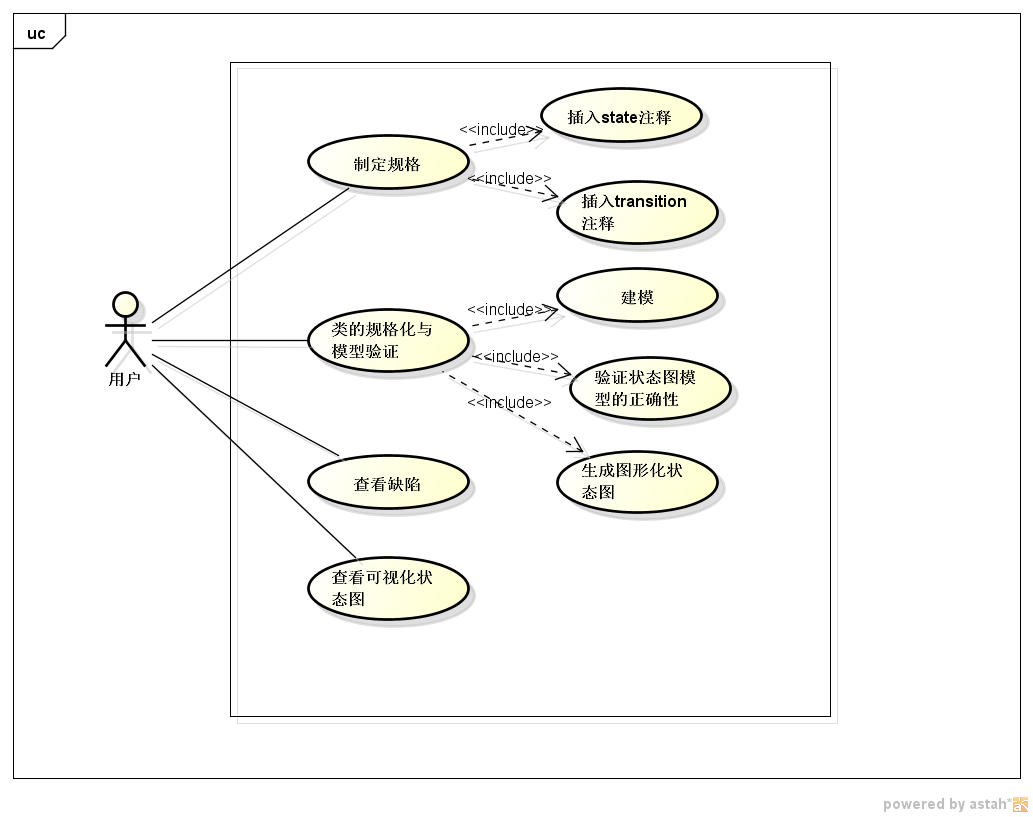
\includegraphics[width=3.6in]{img/2.PNG}
  \end{figure}
\end{frame}
\subsection{概要设计}
\begin{frame}{逻辑视图}
  \begin{figure}[H]
  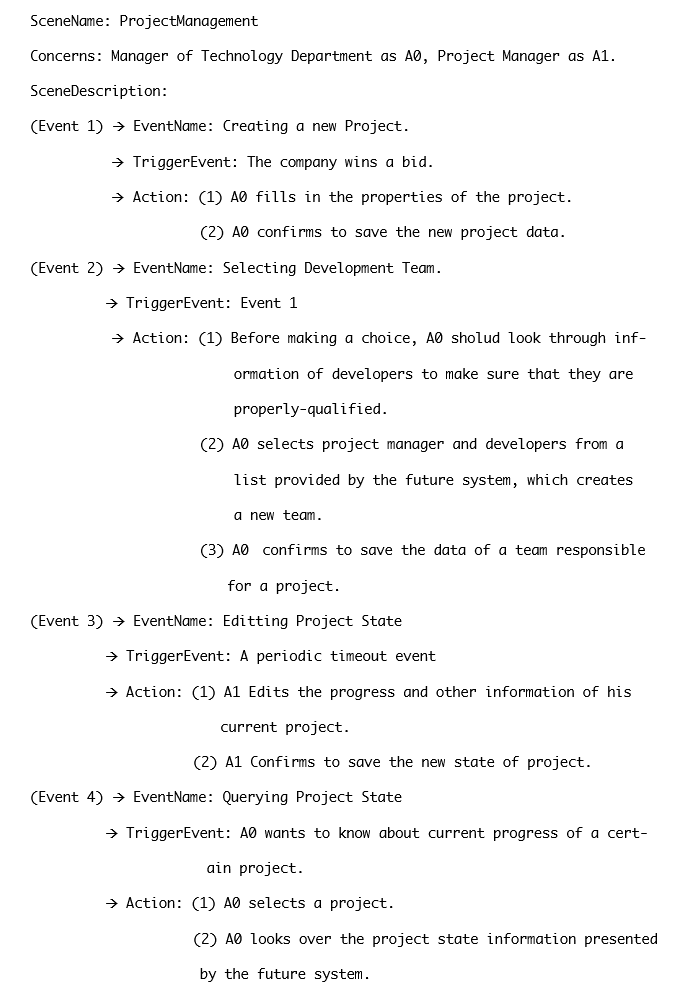
\includegraphics[width=3.6in]{img/3.bmp}
  \end{figure}
\end{frame}
\begin{frame}{协作视图}
  \begin{figure}[H]
  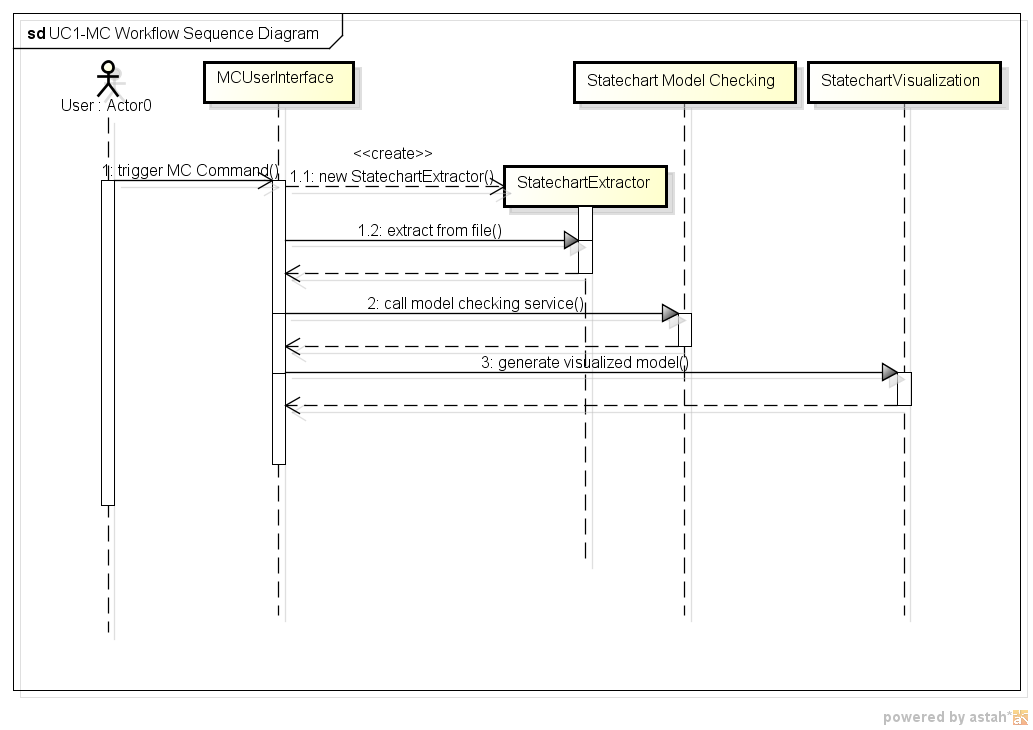
\includegraphics[width=3.6in]{img/4.PNG}
  \end{figure}
\end{frame}

\section{状态图可视化建模的详细设计与实现}
\subsection{详细设计}
\begin{frame}{概述}
  \begin{itemize}
  \item StatechartVisualization+MCUserInterface中的VisualizedStatechartView和MCCommandEntrance。 \pause
  \item 其中StatechartVisualization核心部分由CurveModel实现,ModelDisplayDelegation作为中间层将其与VisualizedStatechartView与MCCommandEntrance这两个模块相连接 \pause
  \end{itemize}
\end{frame}
\begin{frame}{CurveModel模块}
  \begin{figure}[H]
  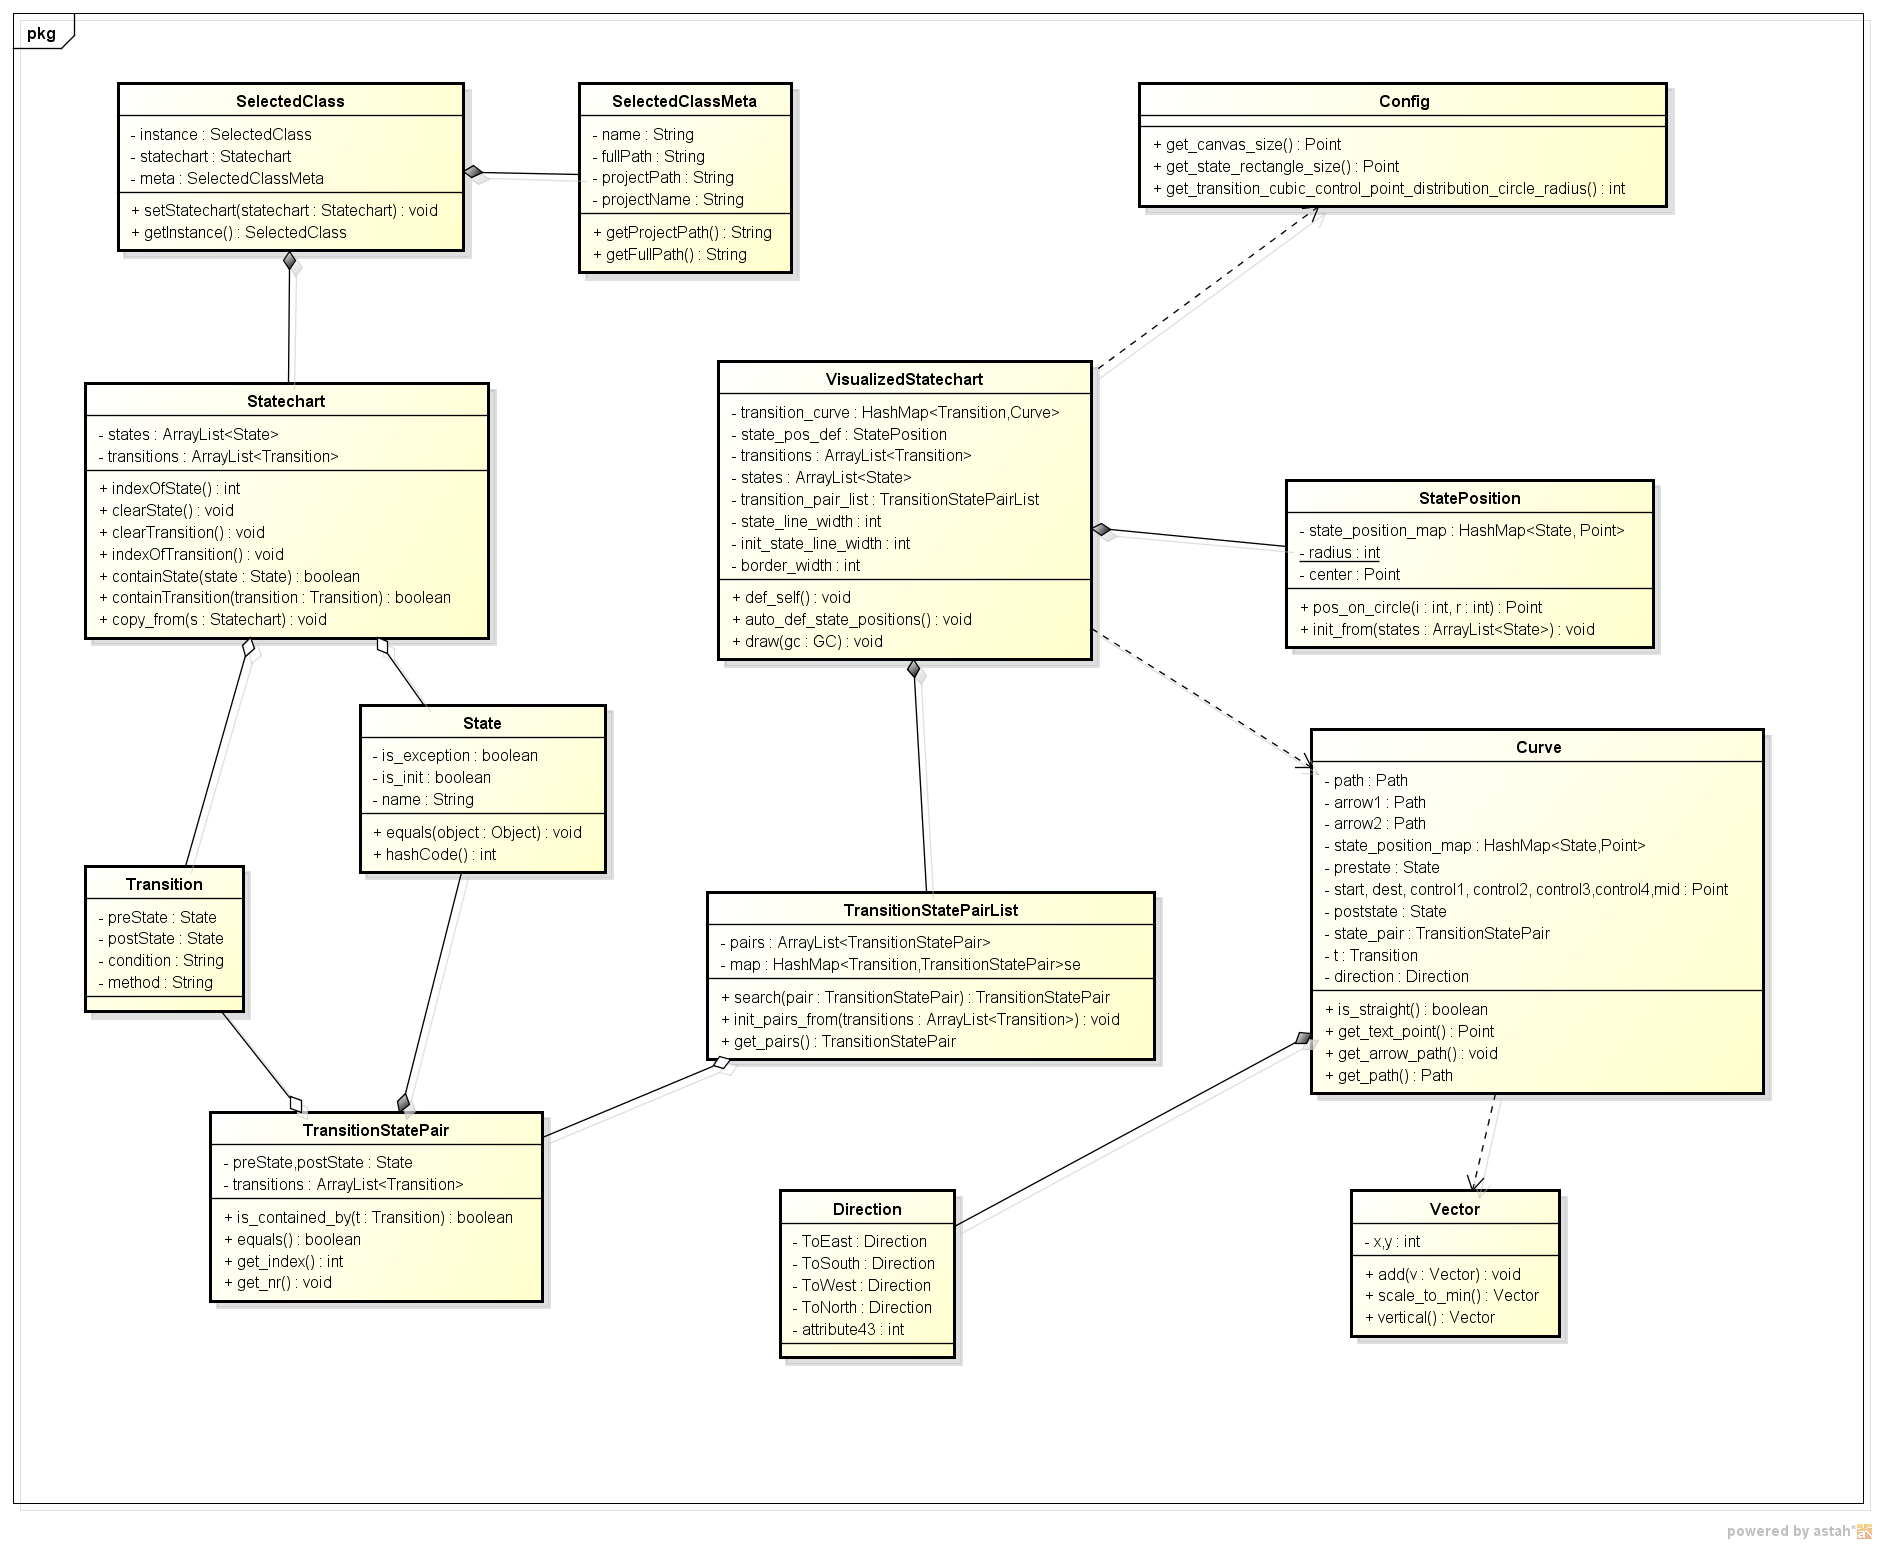
\includegraphics[width=3.6in]{img/5.PNG}
  \end{figure}
\end{frame}
\begin{frame}{MCCommandEntrance,VisualizedStatechartView以及中间件ModelDisplayDelegation}
  \begin{figure}[H]
  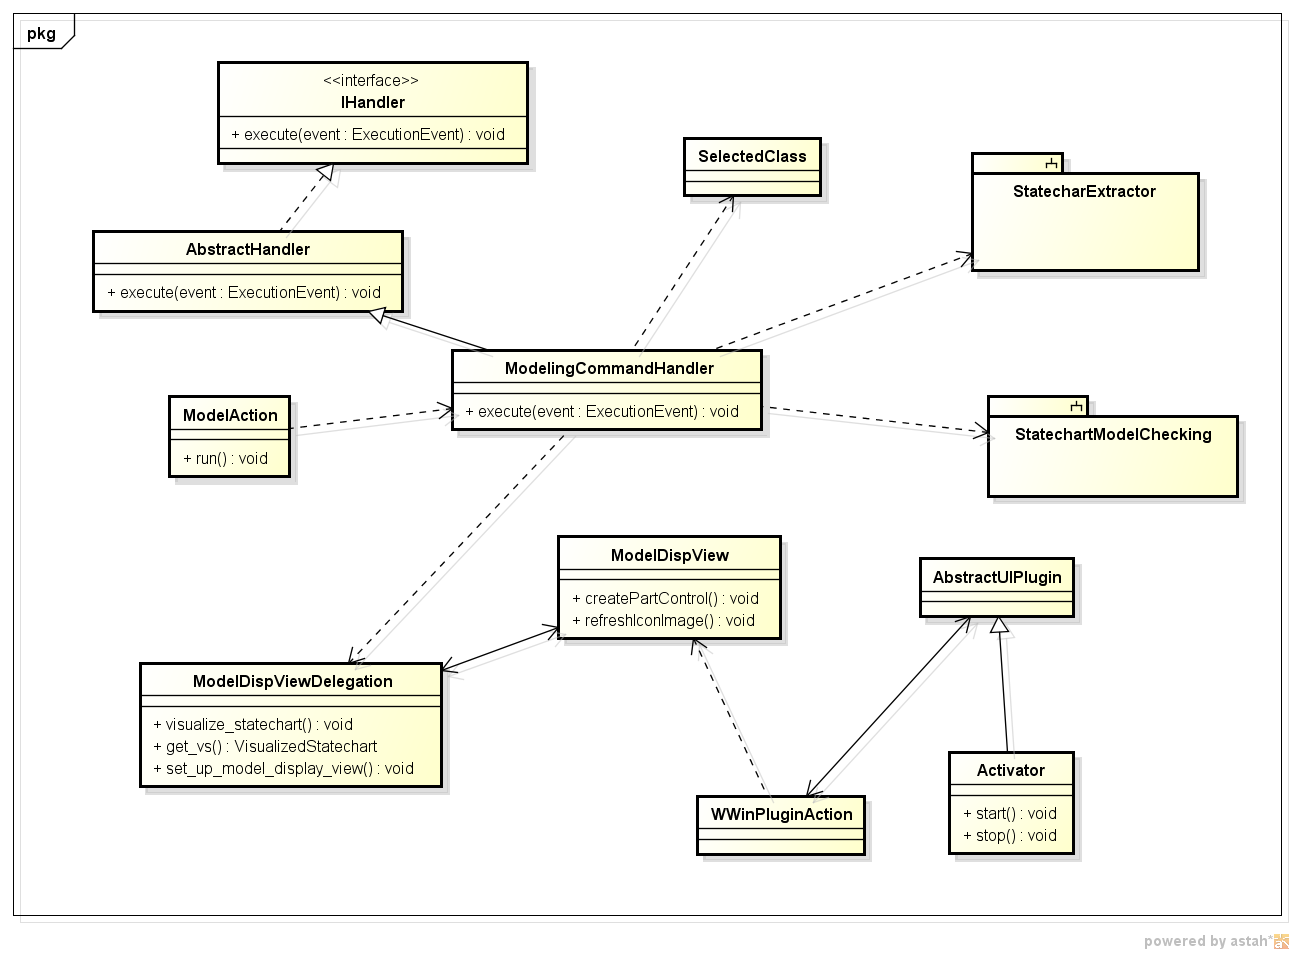
\includegraphics[width=3.6in]{img/6.PNG}
  \end{figure}
\end{frame}
\begin{frame}{CurveModel、ModelDisplayDelegation和MCUserInterface的入口组件调用顺序}
  \begin{figure}[H]
  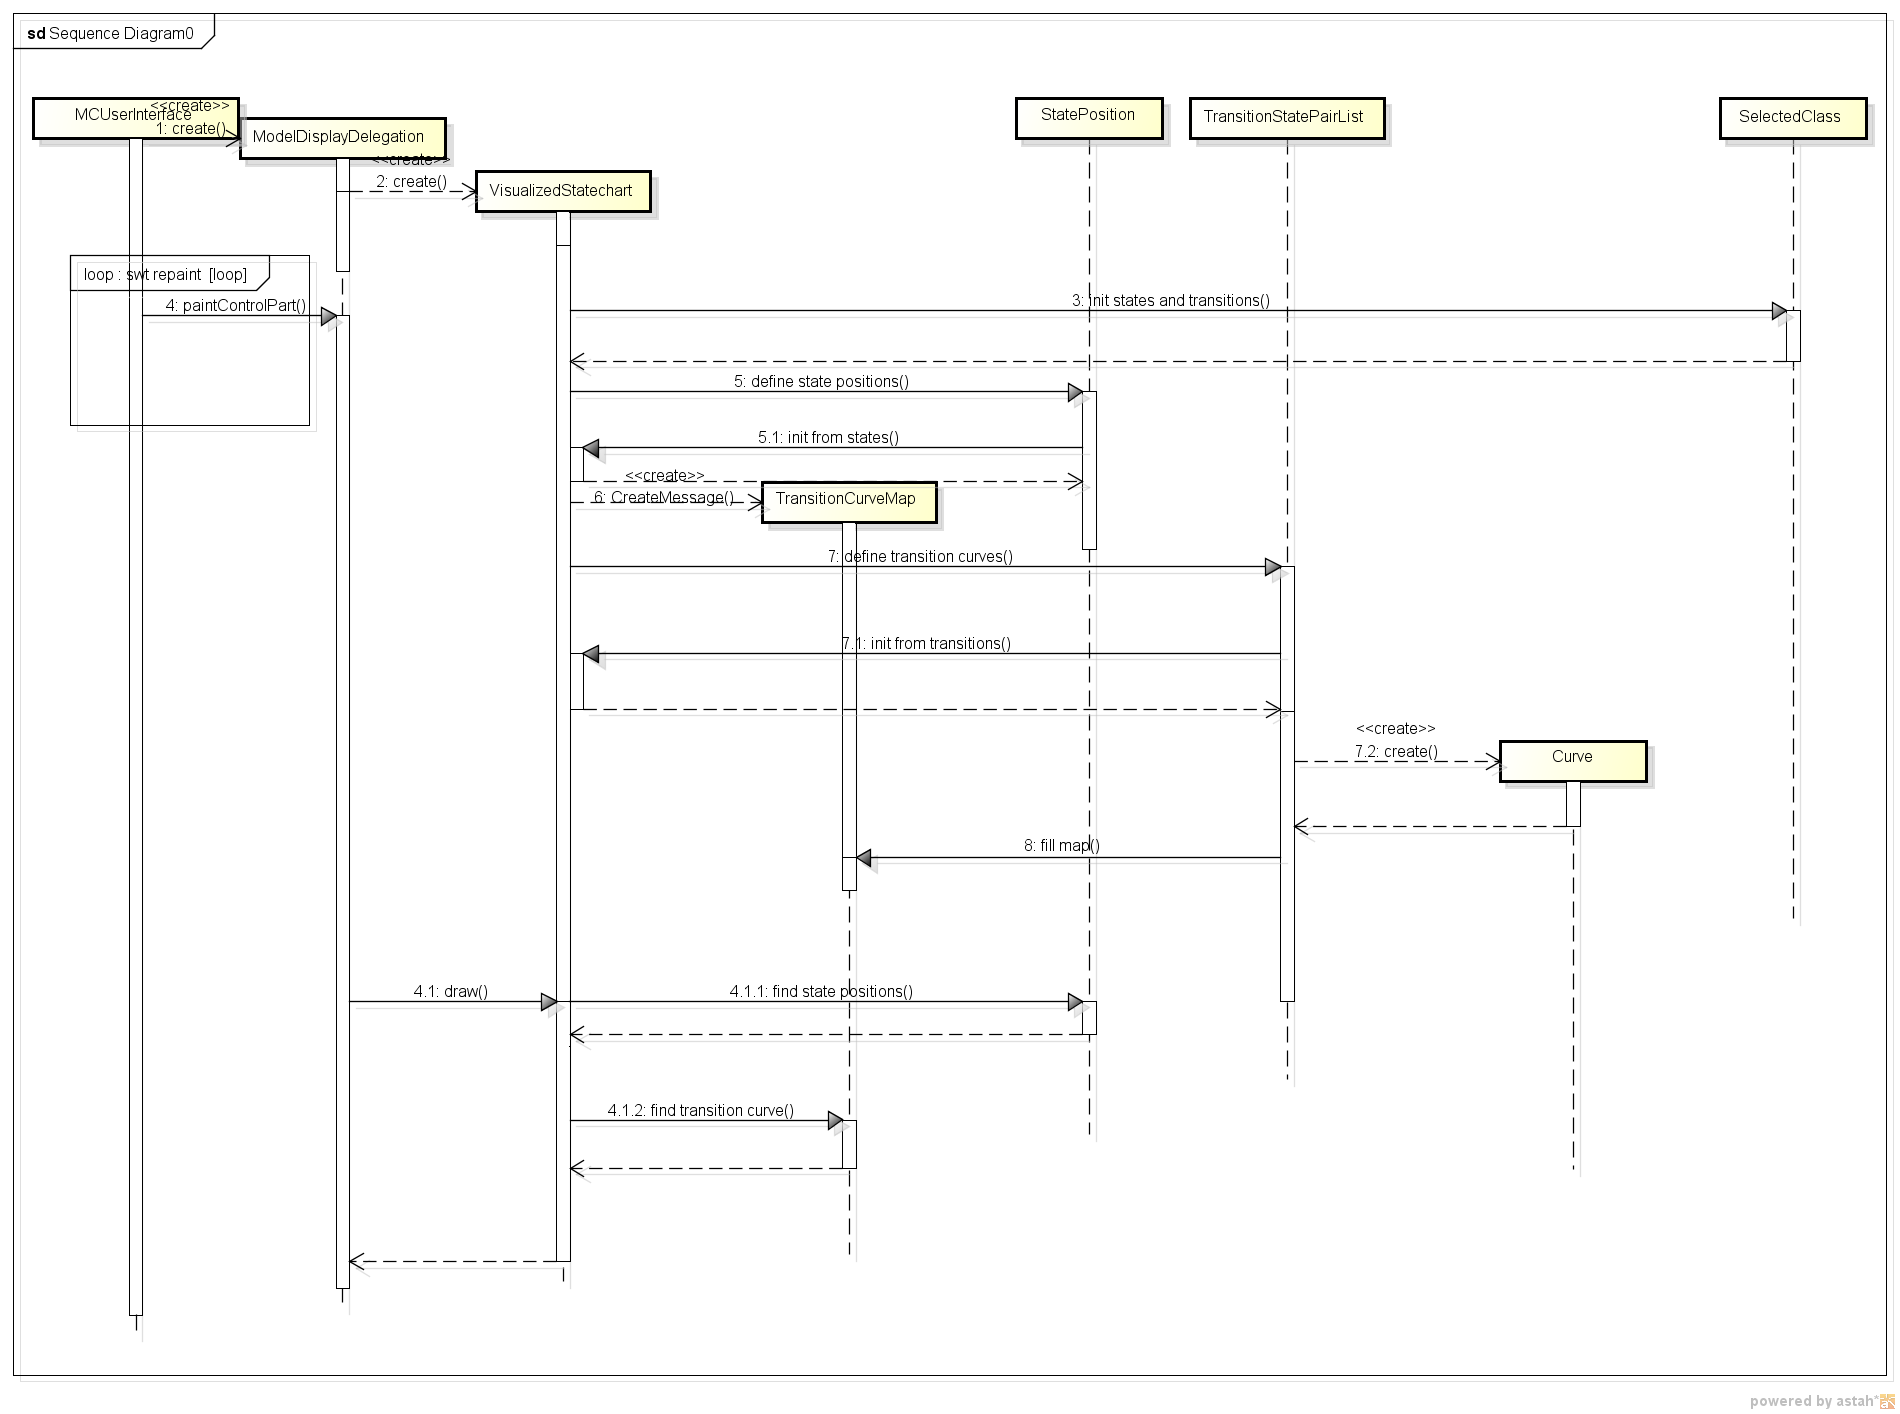
\includegraphics[width=3.6in]{img/7.PNG}
  \end{figure}
\end{frame}

\subsection{重要算法实现}
\begin{frame}{主要步骤}
  \begin{figure}[H]
  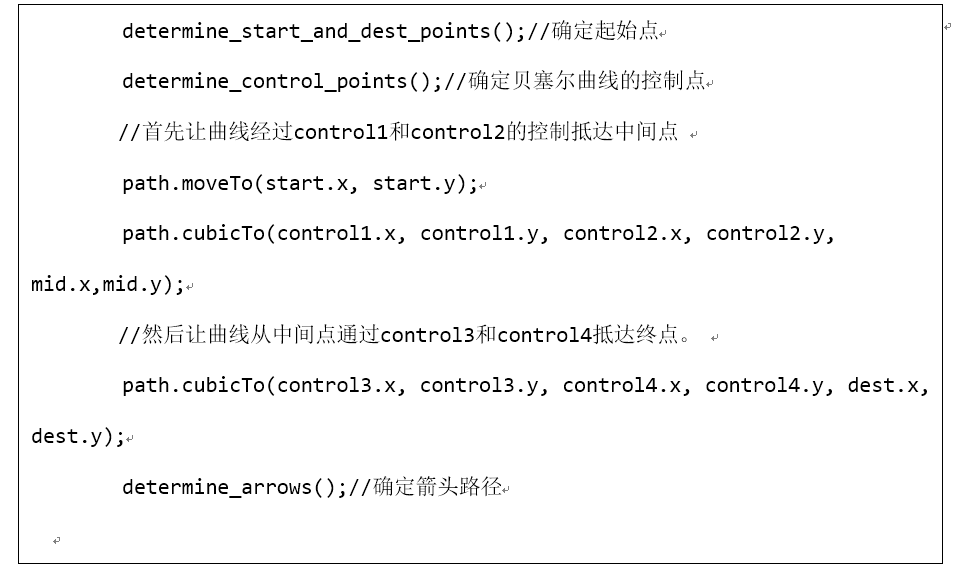
\includegraphics[width=3.6in]{img/8.PNG}
  \end{figure}
\end{frame}

\begin{frame}{重要步骤算法}
  \begin{itemize}
  \item 根据前置状态到后置状态的连线的方向决定起始点位置 \pause
  \item 确定贝塞尔曲线的控制参数:\pause
    \begin{itemize}
    \item Curve模块中使用的变迁路径曲线为2条贝塞尔曲线的拼接版本。\pause
    \item 控制参数:control1、control2、control3、control4、mid、start、dest。\pause
    \item control1位于以起始点为圆心的一个圆上,所有(前置状态,后置状态)相同的变迁的control1都均匀分布在这个圆上,保证变迁曲线在起始点处的切线斜率的分布是均匀的。\pause
    \item 同理所有同类transition的control4也均匀分布在终点为圆心的一个圆上。\pause
    \end{itemize}
  \end{itemize}
\end{frame}

\begin{frame}{重要步骤算法}
  \begin{itemize}
  \item 
    \begin{itemize}
    \item 下一步是确定一个曲线必然经过的点,用于添加文字信息标注曲线方法名、守护条件等相关属性,这个点称为曲线中点。曲线中点被定义为control1和control4的中点,它是第一条贝塞尔曲线的终点和第二条贝塞尔曲线的起点。\pause
    \item 最后确定control2和control3,这两个控制参数不应该扭曲曲线的方向,因此分别取control1和mid的中点,control4和mid的中点。\pause
    \end{itemize}
  \item 生成曲线路径 \pause
  \item 确定箭头,过终点与control4的直线就是位于终点处的切线。 \pause
  \end{itemize}
\end{frame}

\end{document}
